\section{2020 年 10 月 24 日答疑记录}

\subsection{判断两个函数是否相同}

因为函数是由其定义域和对应法则决定的, 所以判断两个函数是否相同也应从这两个方面考虑: 先看定义域是否相同, 若不同, 则两个函数不同; 若相同, 再看表达式能否化为相同的形式. 只有定义域和对应法则都相同的函数才是同一个函数. 另外需要注意, 函数是否相同与其所用的字母无关: 定义域是自变量的取值范围 (一个数集), 对应法则是运算规则, 两者都不涉及表达式中的字母选择. 例如, 

$f(x)=2x+1$ ($x>1$) 与 $g(u)=2u+1$ ($u>1$) 是相同的函数 (仅所用字母不同); 

$f(x)=2x+1$ ($x>1$) 与 $g(u)=2u+1$ ($u>2$) 是不同的函数 (定义域不同);

 $f(x)=2x+1$ ($x>1$) 与 $g(u)=3u+1$ ($u>1$) 也是不同的函数  (对应法则不同).

\begin{example}
    下列各组函数中, \underline{\qquad} 的两个函数为相同的函数.
    
    (1) $f(x)= x^2-2x-1$, $g(s)=s^2-2s-1$;
    
    (2) $f(x)=\dfrac{x}x$, $g(x)=\dfrac1{x^0}$;\qquad
    (3) $f(x)=\sqrt{-x^3}$, $g(x)=x\sqrt{x}$;
    
    (4) $f(x)=x$, $g(x)=\sqrt{x^2}$;\qquad
    (5) $f(x)=\sqrt{x^3}$, $g(x)=x\sqrt{x}$.
\end{example}
\begin{solution}
    (1) $f(x)$ 与 $g(s)$ 定义域均为 $\realnum$, 且对应法则相同, 所以为相同的函数 (仅自变量所用字母不同).
    
    (2) $f(x)$ 与 $g(x)$ 定义域均为 $\{x\mid x\neq 0\}$, 且
    \[f(x)=1,\quad g(x)=\frac11=1,\]
    所以 $f(x)=g(x)$.
    
    (3) 对 $f(x)$, $-x^3\geqslant 0$, 解得 $x\leqslant 0$.
    对 $g(x)$, $x\geqslant 0$. 所以 $f(x)$ 与 $g(x)$ 的定义域不同, 两者为为不同的函数.
    
    (4) $f(x)$ 与 $g(x)$ 的定义域都是 $\realnum$, 但是 $g(x)=|x|\neq f(x)$.
    
    (5) $f(x)$ 与 $g(x)$ 的定义域都是 $[0,+\infty)$, 而
    \[f(x)=\sqrt{x^2\cdot x}=|x|\sqrt{x}\neq g(x),\]
    所以两者为不同的函数.
    
    综上可知, (1)(2) 的两个函数为相同的函数.
\end{solution}
\begin{remark}
    $\sqrt{x^2}=|x|$ 的解释: 当 $x\geqslant 0$ 时, $\sqrt{x^2}=x$; 当 $x< 0$ 时, $\sqrt{x^2}=-x$, 恰好符合 $|x|$ 的定义. 另一种推导为
    \[\sqrt{x^2}= \sqrt{|x|^2}= |x|.\]
    类似的结论还有
    \[\sqrt[3]{x^3}=x\ (\text{没有绝对值符号}),\quad
      \sqrt[4]{x^4}=|x|.\]
\end{remark}

\subsection{分段函数}

分段函数相关的问题, 分段考虑即可.

\begin{example}
    已知函数 $f(x)=\begin{cases}
        2x+1, & x\geqslant 0,\\
        3x^2, & x<0
    \end{cases}$ 且 $f(x_0)=3$, 求实数 $x_0$ 的值.
\end{example}
\begin{solution}
    题中没有给 $x_0$ 的取值范围, 所以需要分类讨论.
    
    (1) 若 $x_0\geqslant 0$, 则 $f(x_0)=3$ 化为 $2x_0+1=3$, 解得 $x_0=1$.
    
    (2) 若 $x_0< 0$, 则 $f(x_0)=3$ 化为 $3x_0^2=3$, 解得 $x_0=\pm1$. 结合前提 $x_0< 0$ 知, $x=-1$.
    
    综上所述, $x_0=1$ 或 $-1$.
\end{solution}

\begin{example}
    求函数 $f(x)=\begin{cases}
        x^2-x+1, & x< 1,\\
        \dfrac1x, & x\geqslant 1
    \end{cases}$ 的值域.
\end{example}
\begin{solution}
    (1) 当 $x<1$ 时, $f(x)=x^2-x+1$ 为二次函数, 对称轴为 $x=\dfrac12$, 所以此时 $f(x)\in\biggl[f\biggl(\dfrac12\biggr),+\infty\biggr)= \biggl[\dfrac34,+\infty\biggr)$.
    
    (2) 当 $x\geqslant 1$ 时, $f(x)=\dfrac1x$ 为反比例函数, 由其图象知, 此时 $f(x)\in(0,f(1)]= (0,1]$.
    
    综上所述, $f(x)$ 的值域为 $\biggl[\dfrac34,+\infty\biggr)\cup (0,1]= (0,+\infty)$.
\end{solution}
\begin{remark}
    反比例函数 $f(x)= \dfrac1x$ ($x\neq 0$) 的图象如下:
    
    \begin{center}
        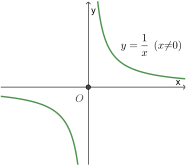
\includegraphics[scale=1]{2020-1108-2300-crop}
    \end{center}
    
    从图象可以看出, 该函数 (1) 在 $(-\infty,0)$ 和 $(0,+\infty)$ 均单调递减; (2) 值域为 $(-\infty,0)\cup (0,+\infty)$; (3) 以 $x$~轴和 $y$~轴为两条渐近线.
\end{remark}
